\documentclass[a4paper,twoside,10pt]{article}

%% Language %%%%%%%%%%%%%%%%%%%%%%%%%%%%%%%%%%%%%%%%%%%%%%%%%
\usepackage[T1]{fontenc}
\usepackage[utf8]{inputenc}
\usepackage[english]{babel}
\usepackage[top=2.5cm, bottom=2.5cm, left=2.5cm, right=2.5cm]{geometry}
\usepackage{scrextend}
\addtokomafont{labelinglabel}{\sffamily}
\usepackage{lmodern} %Type1-font for non-english texts and characters
\usepackage{parskip}
\usepackage{enumitem}

%% Packages for Graphics, Figures & Tables %%%%%%%%%%%%%%%%%%%%%%%%%%
\usepackage{graphicx} %%For loading graphic files
\usepackage{subcaption}
\usepackage{float}
\usepackage{booktabs} %% for top/midrule
\usepackage{textcomp}
\usepackage[table,xcdraw, dvipsnames]{xcolor}
\usepackage{tabularx}
\usepackage{longtable}
\usepackage{makecell}
\usepackage{pdflscape}

%bibliography
\usepackage[round]{natbib}
\bibliographystyle{abbrvnat}
\usepackage{hyperref}
\hypersetup{
    colorlinks=false,
    pdfborder={0 0 0} % Removes the border
}
\usepackage{geometry}

%% Math Packages %%%%%%%%%%%%%%%%%%%%%%%%%%%%%%%%%%%%%%%%%%%%
\usepackage{amsmath}
\usepackage{amsthm}
\usepackage{amsfonts}


%% Line Spacing %%%%%%%%%%%%%%%%%%%%%%%%%%%%%%%%%%%%%%%%%%%%%
\usepackage{setspace}
\onehalfspacing       %% 1,5-spacing
\usepackage{placeins}


\usepackage{titlesec}
\titlespacing{\section}{0pt}{*4}{*1.5} 
\titlespacing{\subsection}{20pt}{*4}{*1.5}
\titlespacing{\subsubsection}{40pt}{*4}{*1.5} 
\titlespacing{\paragraph}{60pt}{*4}{*1.5}
\titlespacing{\subparagraph}{80pt}{*4}{*1.5}


%%%%%%%%%%%%%%%%%%%%%%%%%%%%%%%%%%%%%%%%%%%%%%%%%%%%%%%%%%%%%
%% DOCUMENT
%%%%%%%%%%%%%%%%%%%%%%%%%%%%%%%%%%%%%%%%%%%%%%%%%%%%%%%%%%%%%
\begin{document}

 
\begingroup  
  \centering
\textbf{Title: Long-term abundance time-series of the High Arctic terrestrial vertebrate community of Bylot Island, Nunavut}\\[1.5em]

\textbf{Authors}:\\
 Louis Moisan\textsuperscript{1,2}, Azenor Bideault\textsuperscript{2,3}, Gilles Gauthier\textsuperscript{4}, Éliane Duchesne\textsuperscript{1}, 
 Dominique Fauteux\textsuperscript{5}, Dominique Berteaux\textsuperscript{1}, Pierre Legagneux\textsuperscript{3,6}, Marie-Christine Cadieux \textsuperscript{3} and Joël Bêty\textsuperscript{1}\\[1.5em]

\textbf{Author Affiliations}:\\
\textsuperscript{1} Chaire de Recherche du Canada en Biodiversité Nordique, Centre d’Études Nordiques, Centre de la science de la biodiversité du Québec, Département de biologie, chimie et géographie, Université du Québec à Rimouski, Rimouski, QC, Canada\\
\textsuperscript{2} Chaire de Recherche du Canada en Écologie Intégrative, Centre d’Études Nordiques, Centre de la science de la biodiversité du Québec, Département de Biologie, Université de Sherbrooke, Sherbrooke, QC, Canada\\
\textsuperscript{3} Chaire de Recherche Sentinelle Nord sur l’impact des migrations animales sur les écosystèmes nordiques, Centre d’Études Nordiques, Centre de la science de la biodiversité du Québec, Département de Biologie, Université Laval, Québec, QC, Canada\\
\textsuperscript{4} Centre d’études nordiques, Département de Biologie, Université Laval, Québec, QC, Canada\\
\textsuperscript{5} Centre d’études nordiques, Centre for Arctic Knowledge and Exploration, Canadian Museum of Nature, Ottawa, ON, Canada\\
\textsuperscript{6} Centre d’Études Biologiques de Chizé (CEBC-CNRS), Université de La Rochelle, France 
\\[1.5em]

\textbf{Corresponding Author}:\\
\textit{\href{mailto:louis.moisan.bio@gmail.com}{louis.moisan.bio@gmail.com}}\\
\textit{\href{mailto:joel_bety@uqar.ca}{joel{\textunderscore}bety@uqar.ca}}
\\[1.5em]

\textbf{Open Research statement}:

%%%%%%% !!!! ADD DRYAD adress !!!! %%%%%%%%
Data are publicly available at \url{https://datadryad.org/}.\\[1.5em]
Raw data and codes used to extract the presented data set are publicly available at \url{https://github.com/chaireBioNorth/BYLOT_species_abundance_dataset}.
\endgroup
\newpage


\subsection*{Introduction}
 The composition of ecological communities, defined as the abundance of each species within a given community, is fundamental for understanding patterns and processes in community ecology. Variations in community composition can help to detect spatial patterns linked to environmental variations \citep{kemp1990}, assess temporal trends of different groups of species after disturbances \citep{philippi1998, magurran2007}, and understand food web structures \citep{cohen2003}. Additionally, community composition is essential for modeling the dynamics of ecological communities. Dynamic community modelling allows addressing important issues and questions in ecology, such as: determining the relative strength of top-down versus bottom-up forces in communities \citep{krebs2003,legagneux2014}, assessing the ecological resilience of communities under climate change \citep{griffith2019} and evaluating the cascading effects of invasive species in food web \citep{david2017, goto2020}. Dynamic community modelling can also be applied to address practical challenges, including fishery management (Plagányi, 2007) and the planning of protected areas \citep{okey2004, dahood2020}. 

Modeling food webs requires adjusting trophic flows based on the functional responses of species, which necessitates time series data on the abundance of all species within a community. However, accurately determining the abundance of all species is rarely achievable. Consequently, empirical community models often reduce taxonomic resolution by grouping species into large functional or taxonomic categories. Additionally, food webs consist of species with varying body sizes depending on their trophic level, with top-level species often being highly mobile and having large home ranges \citep{mccann2005}. Therefore, community models must use landscape-wide estimates of species abundance to accurately represent trophic fluxes. Due to these constraints, empirical datasets with high taxonomic resolution that cover entire communities at broad spatial and temporal scales are rare and often include incomplete or rough estimates.

The composition of ecological communities is influenced by various factors acting at different temporal and spatial scales, leading to noisy data and emphasizing the need for long-term data sets \citep{magurran2010, lindenmayer2012}. Species abundances are influenced by stochastic effects \citep{hubbell2001}, environmental changes (e.g., climate warming), and species interactions, contributing to data variability. For instance, the composition of a community could be driven simultaneously by intra-annual seasonal variations, multi-year cyclic variations (e.g., El Niño) and slow but directional long-term variations in the environment \citep{brown1990, snyder2006}. Therefore, long-term data series are required to untangle the relative effects of diverse abiotic and biotic factors on community composition \citep{magurran2010, lindenmayer2012}.

Arctic environments are highly valuable systems for studying community patterns and processes due to their relatively low species richness \citep{payer2013, legagneux2014}. However, logistical challenges in the Arctic limit the number of long-term biodiversity monitoring programs. Hence, the small number of Arctic communities with long-term monitoring serve as highly valuable sites for holistic and empirical community studies. Datasets on terrestrial communities are notably scarce, and this scarcity extends to Arctic communities as well \citep{ims2013}. 

Within terrestrial Arctic sites, the south plain of Bylot Island in the Canadian High Arctic (\textbf{Figure \ref{figure:food_web}}) hosts one of the longest and most intensive biodiversity monitoring programs \citep{gauthier2024a}. Monitoring on Bylot Island began in 1989 with a focus on the snow goose and it gradually expanded to other species over time. Currently, the program encompasses all significant vertebrate species in the community with continuous monitoring spanning more than a decade \citep{gauthier2024a}. Monitoring is also conducted at multiple spatial scales, including intensive and systematic observations conducted across a landscape spanning approximately 400 km\textsuperscript{2}. This approach allows the scaling of local density measurements to the landscape level when required and facilitates the estimation of abundance for less common and rare species. 

Previous work based on the tundra community of Bylot Island  has already produced several influential papers \citep{gauthier2011, legagneux2012, legagneux2014,hutchison2020, duchesne2021, gauthier2024b}. These studies showed that tundra communities may experience stronger top-down regulation than bottom-up regulation \citep{legagneux2012, legagneux2014}. They also revealed a heterogeneous response of trophic levels to climate warming \citep{gauthier2013} and highlighted the effects of indirect trophic interactions on the occurrence of species across the landscape \citep{duchesne2021}. However, those earlier papers were built on data from relatively short time series, they were not always scaled at the landscape level, and some species or functional groups were lacking abundance estimates. With over a decade of additional community-wide monitoring compared to earlier studies, our goal is to synthesize and upscale the data collected on the Bylot Island community since the 1990s to the landscape level. This synthesis aims to provide readily accessible annual time series (or mean values in some cases) of abundance and biomass for all vertebrate species in a tundra landscape, covering approximately 400 km\textsuperscript{2}. 

\begin{figure}[H]
\centering
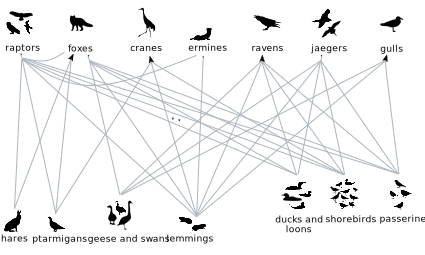
\includegraphics[width=0.75\linewidth]{figures/food_web.pdf} 
\caption{Synthetic vertebrate food web of the south plain of Bylot Island (figure adapted from \citet{gauthier2011}.}
\label{figure:food_web}
\end{figure}

\subsection*{Objective}
Our main objective is to provide readily accessible, long-term time series of annual abundances of all vertebrate species within the Arctic terrestrial community of Bylot Island during the breeding season (May to August). This includes both breeding and non-breeding individuals that stay in the study area for a significant period of time, and excludes non-breeding individuals that stop for only a few days during their migration. Our focus extends to estimating abundances at the landscape scale, enabling the study of community and ecosystem dynamics, trophic interactions and the impacts of global changes on high-latitude environments. Additionally, we aim to provide the average body mass for each species in the community, enabling the conversion of abundances into biomasses.
\newpage


\section*{\textcolor{Blue}{Class I. Data Set Descriptors}}
    \section*{A. Data set identity} Long-term abundance time-series of the High Arctic terrestrial vertebrate community of Bylot Island, Nunavut
    \section*{B. Data set identification codes}
     \texttt{BYLOT-species\_taxonomy.csv}\\
     \texttt{BYLOT-species\_abundance.csv}\\
     \texttt{BYLOT-mean\_species\_abundance.csv}\\
     \texttt{BYLOT-mean\_species\_body\_mass.csv}\\
     \texttt{BYLOT-interannual\_variation\_nest\_density.csv}\\
     
    \section*{C. Data set description}
		\subsection*{1. Originators}
		\textbf{Gilles Gauthier}, Centre d’études nordiques, Département de Biologie, Université Laval, Québec, QC, Canada\\
  		\textbf{Joël Bêty},  Chaire de Recherche du Canada en Biodiversité Nordique, Centre d’Études Nordiques, Centre de la science de la biodiversité du Québec, Département de biologie, chimie et géographie, Université du Québec à Rimouski, Rimouski, QC, Canada \\
  		\textbf{Pierre Legagneux}, Chaire de Recherche Sentinelle Nord sur l’impact des migrations animales sur les écosystèmes nordiques, Centre d’Études Nordiques, Centre de la science de la biodiversité du Québec, Centre d’Études Biologiques de Chizé (CEBC-CNRS) Département de Biologie, Université Laval, Québec, QC, Canada
  		
		\subsection*{2. Abstract}
Arctic ecosystems present unique opportunities for community-wide monitoring, in part due to their relatively low species richness. However, conducting research in these remote environments poses significant logistical challenges, resulting in long-term monitoring being exceedingly rare. Here, we focus on the long-term, intensive ecological monitoring efforts conducted on the south plain of Bylot Island (almost 400 km\textsuperscript{2}, Nunavut, Canada), which has generated a remarkable dataset spanning up to 30 years, a rarity in tundra ecosystems. Our goal is to synthesize this dataset and upscale vertebrate abundance data at the landscape level, a prerequisite to conduct community-level analyses. We have standardized data obtained with different field methods to provide readily usable long-term time series of abundance for 35 vertebrate species (30 birds and 5 mammals) present in the study system. Monitoring data includes intensive capture-mark-recapture density estimates of lemmings on trapping grids, systematic or opportunistic nest monitoring conducted across the entire study area or within specific plots for all bird species, transects of vertebrate counts distributed throughout the study area, daily incidental observations of vertebrates and satellite tracking of fox movements. Annual abundance of species was estimated at the landscape level, accounting for spatial variations. Furthermore, we provide body masses for each species, derived from empirical onsite measurements for 18 species and from the literature for the remaining species. Body mass is essential to convert species abundance into biomass for studies of trophic fluxes and ecosystem processes. Our dataset provides a unique opportunity for holistic empirical studies of ecological communities, allowing a deeper understanding of community structure and dynamics. Considering that the study site is a pristine and protected area that has experienced minimal anthropogenic impact, it can also provide an ideal baseline for investigating the impacts of global changes on high-latitude terrestrial ecosystems.


   \section*{D. Key words/phrases}
 Bylot Island, Canadian Arctic, Arctic tundra, 1993-2023, long-term monitoring, biodiversity monitoring, community composition, species abundance, species density, species biomass, species body mass, food web
  \newpage

  
\section*{\textcolor{Blue}{Class II. Research origin descriptors}}
    \section*{A. Overall project description}
    \subsection*{1. Identity} Understanding the structure and dynamics of Arctic terrestrial vertebrate communities

	\subsection*{2. Originators:}	
  	\textbf{Gilles Gauthier}, Centre d’études nordiques, Département de Biologie, Université Laval, Québec, QC, Canada\\
  		\textbf{Joël Bêty},  Chaire de Recherche du Canada en Biodiversité Nordique, Centre d’Études Nordiques, Centre de la science de la biodiversité du Québec, Département de biologie, chimie et géographie, Université du Québec à Rimouski, Rimouski, QC, Canada \\
  		\textbf{Pierre Legagneux}, Chaire de Recherche Sentinelle Nord sur l’impact des migrations animales sur les écosystèmes nordiques, Centre d’Études Nordiques, Centre de la science de la biodiversité du Québec, Centre d’Études Biologiques de Chizé (CEBC-CNRS) Département de Biologie, Université Laval, Québec, QC, Canada
	
	\subsection*{3. Period of study} 1989 - continuing
	
	\subsection*{4. Objectives}
       i) Understand the factors that shape the structure and drive the dynamics of Arctic terrestrial vertebrate communities.\\
       ii) Predict the effects of current global environmental changes on the structure and dynamics of Arctic terrestrial vertebrate communities.
       
     \subsection*{5. Abstract}
        Arctic terrestrial vertebrate communities present low species richness, making those relatively simple communities ideal for studying ecological patterns and dynamics in terrestrial environments. Although, they present complex networks of interacting species, extreme seasonal changes of environmental conditions and a large portion of migratory species, which make challenging the identification of the key factors that shape their structure and dynamics. In the face of rapid global environmental changes, it is crucial to have a comprehensive understanding of the key processes shaping Arctic terrestrial communities structure and dynamics in order to predict how global changes will impact them in the future. Our research emphasizes long-term biodiversity monitoring, a community-wide perspective and food web modeling to achieve this understanding.
       
      \subsection*{6. Sources of funding}
Natural Sciences and Engineering Research Council of Canada, Fonds Québécois de Recherche Nature et Technologies, Centre d'études nordiques, Natural Resources Canada (Polar Continental Shelf Program), Network of Centers of Excellence Canada (ArcticNet), Canada First Research Excellence Fund (Sentinel North Program), Polar Knowledge Canada, Environment and Climate Change Canada, Canada Foundation for Innovation, Parks Canada Agency, International Polar Year program of the Government of Canada, Crown–Indigenous Relations and Northern Affairs Canada (Northern Contaminant Program), Duck Unlimited Canada, Kenneth M. Molson Foundation (Kenneth M. Molson Foundation’s donation for wildlife research, conservation, and habitat), Garfield Weston Foundation, First Air——Canadian North, Nunavut Wildlife Management Board, Université Laval, Université du Québec à Rimouski
\newpage
        
    \section*{B. Specific subproject description}
     	\subsection*{1. Site description}
 			\subsubsection*{a. Site type}
  The study area (389 km\textsuperscript{2}) represents a relatively productive tundra ecosystem in the eastern Canadian High-Arctic.An important biological characteristic of the area is the presence of a large snow goose (scientific names of most vertebrate species can be found in \textbf{Table \ref{table:species_name_strategy}}) colony of around 25 000 breeding pairs \citep{reed2002} spanning approximately 70 km\textsuperscript{2}. The vertebrate community within the study area comprises 30 bird species, with 29 of them being migratory or partially migratory, along with 5 mammal species (\textbf{Table \ref{table:species_name_strategy}}; \citet{moisan2023, gauthier2024a}). The study area experiences significant temporal fluctuations in the population of small mammals (lemmings), which in turn impact the occurrence and abundance of their avian and mammalian predators such as snowy owls, rough-legged hawks, long-tailed jaegers, ermines and Arctic foxes \citep{legagneux2012}. We exclude occasional visitors, namely: i) species lacking confirmed breeding occurrences on the study site, ii) species observed solely within a single year, and iii) species primarily breeding and foraging in nearby marine or coastal habitats \citep{moisan2023}. The case of the red fox (\textit{Vulpes vulpes}) was ambiguous. While the presence of a breeding pair has been confirmed in the study area \citep{lai2022}, the extent of population establishment remains unclear and sightings are rare. Therefore, we decided to exclude this species.

         		% latex table generated in R 4.4.1 by xtable 1.8-4 package
% Thu Sep 19 09:15:03 2024
\begin{table}[ht]
\centering
\caption{Species composition of the vertebrate community of Bylot Island with the corresponding annual cycle strategy (i.e., resident, partial migrant, migrant).} 
\label{table:species_name_strategy}
\begingroup\fontsize{10pt}{10pt}\selectfont
\begin{tabularx}{0.95\textwidth}{llll}
  \hline
Functional group & Scientific name & Name & Annual cycle strategy \\ 
  \hline
ducks and loons  & Somateria spectabilis & king eider & migrant \\ 
  ducks and loons  & Clangula hyemalis & long-tailed duck & migrant \\ 
  ducks and loons  & Gavia pacifica & Pacific loon & migrant \\ 
  ducks and loons  & Gavia stellata & red-throated loon & migrant \\ 
  geese and swans  & Branta hutchinsii & cackling goose & migrant \\ 
  geese and swans  & Anser caerulescens & snow goose & migrant \\ 
  geese and swans  & Cygnus columbianus & tundra swan & migrant \\ 
  raptors  & Buteo lagopus & rough-legged hawk & migrant \\ 
  raptors  & Falco peregrinus & peregrine falcon & migrant \\ 
  raptors  & Bubo scandiacus & snowy owl & migrant \\ 
  ptarmigans  & Lagopus muta & rock ptarmigan & resident \\ 
  cranes  & Antigone canadensis & sandhill crane & migrant \\ 
  shorebirds  & Pluvialis dominica & American golden-plover & migrant \\ 
  shorebirds  & Pluvialis squatarola & black-bellied plover & migrant \\ 
  shorebirds  & Charadrius hiaticula & common-ringed plover & migrant \\ 
  shorebirds  & Arenaria interpres & ruddy turnstone & migrant \\ 
  shorebirds  & Calidris canutus & red knot & migrant \\ 
  shorebirds  & Calidris melanotos & pectoral sandpiper & migrant \\ 
  shorebirds  & Calidris bairdii & Baird's sandpiper & migrant \\ 
  shorebirds  & Calidris fuscicollis & white-rumped sandpiper & migrant \\ 
  shorebirds  & Calidris subruficollis & buff-breasted sandpiper & migrant \\ 
  shorebirds  & Phalaropus fulicarius & red phalarope & migrant \\ 
  gulls  & Larus hyperboreus & glaucous gull & migrant \\ 
  jaegers  & Stercorarius longicaudus & long-tailed jaeger & migrant \\ 
  jaegers  & Stercorarius parasiticus & parasitic jaeger & migrant \\ 
  ravens  & Corvus corax & common raven & partial migrant \\ 
  passerines  & Eremophila alpestris & horned lark & migrant \\ 
  passerines  & Anthus rubescens & American pipit & migrant \\ 
  passerines  & Calcarius lapponicus & Lapland longspur & migrant \\ 
  passerines  & Plectrophenax nivalis & snow bunting & migrant \\ 
  lemmings  & Lemmus trimucronatus & brown lemming & resident \\ 
  lemmings  & Dicrostonyx groenlandicus & collared lemming & resident \\ 
  hares  & Lepus arcticus & Arctic hare & resident \\ 
  ermines  & Mustela richardsonii & ermine & resident \\ 
  foxes  & Vulpes lagopus & Arctic fox & partial migrant \\ 
   \hline
\end{tabularx}
\endgroup
\end{table}

%label-> table:species_name_strategy
\newpage
            	\subsubsection*{b. Geography} Our 463 km\textsuperscript{2} study area is located on the southern plain of Bylot Island, Nunavut, Canada (72.889 N, -79.906 W; \textbf{Figure \ref{figure:zones}}).
            	\subsubsection*{c. Habitat}  The study area comprises a combination of mesic tundra mainly on hills (64 \%), upland plateaus of sedimentary rock with drier/rockier habitat at higher elevation (20 \%), low-lying wetlands interspersed with ponds (10 \%) and larger bodies of water such as lakes and rivers (6 \%).
            	\subsubsection*{d. Geology} see \citet{klassen1993} for a complete and detailed description of the geology of the study area.
            	\subsubsection*{e. Hydrology} Wetlands were delineated by photo-interpretation of high-resolution satellite images (30 cm; Ouellet, unpublished data), whereas lakes were delineated with aerial photos and rivers with google satellite images, resulting in a coarser delineation.
            	\subsubsection*{f. Site history} see \citet{gauthier2024a, gauthier2024b}  for a complete and detailed history of the site.
            	\subsubsection*{g. Climate} The mean temperature in July is 6°C, and the study area typically remains free of snow from mid-June to late September \citep{gauthier2013}. The climate of the southern plain of Bylot Island is generally milder than that of the surrounding latitudes, as the plain present a southern exposure and the mountains to the north protect the plain from cold northerly winds. \citep{gauthier2024a}.
 \newpage
       
      	\subsection*{2. Experimental or sampling design}
        		\subsubsection*{a. Permanent plots}
The study area is divided into 9 zones based on the sampling method and the level of field effort applied in each zone (\textbf{Figure \ref{figure:zones}}). Long-term monitoring of the community began in the 1990s in the Qarlikturvik valley \citep{gauthier2013, gauthier2024a}, which represents the zone of the study area with the highest annual sampling effort. Within the Qarlikturvik valley, the sampling is concentrated on the southern side of the glacial river (\textbf{Figure \ref{figure:qarlikturvik_valley}}), where the main research infrastructure is located. Another zone with extensive sampling efforts is Camp 2, located at the core of the snow goose colony, where the primary focus is to monitor snow goose nests. However, nests of many other avian species are also monitored within and around the colony in this zone. Camp 3, Pointe Dufour, Goose Point, and Malaview are zones where intensive sampling efforts are conducted annually, albeit for a relatively brief period (approximately one week) during the breeding season of most species \citep{gauthier2024a}. The upland zones in the study area (defined as areas approximately 300 meters above sea level or more) are the Black Plateau, Southern Plateau, and Camp 3 Plateau. These zones are primarily visited to assess raptor nesting activity \citep{beardsell2016}. The zone between the Qarlikturvik valley and Camp 3 received very little sampling effort and is therefore excluded from the study area.

\begin{figure}
\centering
  \includegraphics[width=0.8\textwidth, angle=0]{figures/zones_study_area.pdf}
   \caption{Map of the different zones (colored polygons) of the 463 km\textsuperscript{2} study area located on the southern plain of Bylot Island, Nunavut Canada. The outline of the snow goose colony is presented with white dash; we used the outline of the colony in 2015 since it represents an average colony area (67 km\textsuperscript{2}).}
  \label{figure:zones}
\end{figure}

\begin{figure}
\centering
  \includegraphics[width=0.8\textwidth, angle=0]{figures/qarlikturvik_valley.pdf}
  \vspace{-70pt} % Reduce space between figure and caption
  \caption{Intensive nests searching plots (8 km\textsuperscript{2} and 2 km\textsuperscript{2}) located in the Qarlikturvik valley.}
 \label{figure:qarlikturvik_valley}
\end{figure}
\newpage

		\subsubsection*{b. Avian nest monitoring}
Avian nest monitoring was conducted annually except in 2020 and 2021 due to logistical constraints imposed by the COVID-19 pandemic. Systematic nest monitoring refers here to a systematic sampling approach aimed at documenting all nests within a specified area. Monitoring is considered opportunistic when there is a chance that some nests might not have been detected within a specific area. Nest densities derived from nest sampling could be underestimated due to early nest failure (i.e., failure that happened before our sampling period).

% latex table generated in R 4.4.0 by xtable 1.8-4 package
% Fri Jun 28 12:52:35 2024
\begin{table}[ht]
\centering
\caption{Summary of vertebrate species monitoring in the Bylot Island study area. In this paper, we excluded certain years for specific species due to reduced sampling efforts. As a result, duration of times series presented here may differ slightly from those in in Gauthier et al. (2024b).} 
\label{table:species_year_monitoring}
\begingroup\fontsize{8pt}{10pt}\selectfont
\begin{tabularx}{\textwidth}{lllll}
  \hline
Species & Zone & Years & Monitoring & References \\ 
  \hline
snow goose & camp 2 & 1999-2019, 2023 & systematic & Gauthier et Cadieux, 2020 \\ 
  rough-legged hawk & qarlikt., black \& south plat. & 2007-2019, 2022 & systematic & Gauthier et al., 2020 \\ 
  peregrine falcon & qarlikt., black \& south plat. & 2007-2019, 2022 & systematic & Gauthier et al., 2020 \\ 
  snowy owl & qarlikt., black \& south plat. & 1996-2019, 2023 & systematic & Gauthier et al., 2020 \\ 
  Baird's sandpiper & qarlikturvik (2x1 km plot) & 2005-2019, 2022-2023 & systematic & Bêty, 2020 \\ 
  Lapland longspur & qarlikturvik (2x1 km plot) & 2005-2019, 2022-2023 & systematic & Gauthier and Bêty, 2020 \\ 
  king eider & qarlikturvik (4x2 km plot) & 2005-2019, 2022 & opportunistic & unpublished data \\ 
  long-tailed duck & qarlikturvik (4x2 km plot) & 2005-2019, 2022 & opportunistic & unpublished data \\ 
  rock ptarmigan & qarlikturvik (4x2 km plot) & 2005-2019, 2022 & opportunistic & unpublished data \\ 
  sandhill crane & qarlikturvik (4x2 km plot) & 2005-2019, 2022 & opportunistic & unpublished data \\ 
  brown lemming & qarlikturvik (trapping grids) & 1995-2019, 2021-2022 & systematic & Gauthier, 2020 \\ 
  collared lemming & qarlikturvik (trapping grids) & 1995-2019, 2021-2022 & systematic & Gauthier, 2020 \\ 
  Pacific loon & qarlikturvik valley & 2004-2019, 2022 & systematic & unpublished data \\ 
  red-throated loon & qarlikturvik valley & 2004-2019, 2022 & systematic & unpublished data \\ 
  cackling goose & qarlikturvik valley & 2004-2019, 2022-2023 & systematic & unpublished data \\ 
  tundra swan & qarlikturvik valley & 2004-2019, 2022 & systematic & unpublished data \\ 
  glaucous gull & qarlikturvik valley & 2004-2019, 2022 & systematic & Gauthier et al., 2020 \\ 
  long-tailed jaeger & qarlikturvik valley & 2004-2019, 2022 & systematic & Gauthier et al., 2020 \\ 
  parasitic jaeger & qarlikturvik valley & 2004-2019, 2022 & systematic & unpublished data \\ 
  Pacific loon & whole study area & 2017-2019, 2022 & systematic & Duchesne et al., 2021 \\ 
  red-throated loon & whole study area & 2017-2019, 2022 & systematic & Duchesne et al., 2021 \\ 
  cackling goose & whole study area & 2017-2019, 2022-2023 & systematic & Duchesne et al., 2021 \\ 
  tundra swan & whole study area & 2017-2019, 2022 & systematic & Duchesne et al., 2021 \\ 
  rough-legged hawk & whole study area & 2013-2019, 2022 & systematic & Gauthier et al., 2020 \\ 
  peregrine falcon & whole study area & 2013-2019, 2022  & systematic & Gauthier et al., 2020 \\ 
  snowy owl & whole study area & 2012-2019, 2022-2023 & systematic & Gauthier et al., 2020 \\ 
  common-ringed plover & whole study area & 2015-2017 & systematic & Bêty, 2020 \\ 
  glaucous gull & whole study area & 2017-2019, 2022 & systematic & Gauthier et al., 2020 \\ 
  parasitic jaeger & whole study area & 2009-2019, 2022 & opportunistic & unpublished data \\ 
  common raven & whole study area & 2013-2019, 2022 & systematic & unpublished data \\ 
  ermine & whole study area & 1993-2019 & opportunistic & Bolduc et al., 2023 \\ 
  Arctic fox & whole study area & 2008-2016 & systematic & Dulude-de Broin et al., 2023 \\ 
   \hline
\end{tabularx}
\endgroup
\end{table}

%label-> table:species_year_monitoring


	\begin{enumerate}[label=\roman*]
	\item[] \textit{\textbf{Pacific loon, red-throated loon, cackling goose, tundra swan and glaucous gull}}\\
	Since 2004, systematic searches of wetland areas have been conducted on the southern side of the glacial river in the Qarlikturvik Valley, and since 2017, in other zones of the study area. This sampling aimed to find all nests of the cackling goose and the glaucous gull. Nest locations of other large wetland-nesting species, including the tundra swan, the red-throated loon and the Pacific loon, were also noted, as these species nest in the same habitat \citep{duchesne2021,gauthier2024a}. Each year, all known or potential nesting sites were revisited. Observers detected nests by walking and scanning around ponds and lakeshores to identify any active nesting sites. These large species can be seen from a relatively long distance sitting on the nest or when flushing from the nest. Most of them (geese, swans and gulls) can also reveal their presence with alarm calls or nest defense displays. We are confident that nest detection probability was high for these species given the open landscape.\\
	
	\item[] \textit{\textbf{Snow goose}}\\
	Snow geese nest in a large colony in the study area (\textbf{Figure \ref{figure:zones}}), but also in small aggregations distributed on the island, especially in years when snowy owls are nesting \citep{lepage1996,reed2002}. Since 1994, goose nests were systematically monitored on a 0.24 km\textsuperscript{2} wetland at the center of the colony. Since 1999, nests were also systematically monitored on a variable number of plots, measuring 0.01 km\textsuperscript{2} in wetland habitat and 0.04 km\textsuperscript{2} in mesic habitat, randomly distributed throughout the goose colony \citep{gauthier2020goose}. The total area covered by the randomly distributed plots averaged 0.79 \textpm{0.37} km\textsuperscript{2} per year. From 2010 onwards, except in 2020 and 2021, we traced the approximate boundary of the goose colony using a GPS receiver aboard a helicopter flying along the colony border \citep{duchesne2021}.
	
	\item[] \textit{\textbf{Rough-legged hawk, peregrine falcon and common raven}}\\
	Peregrine falcons, rough-legged hawks and common ravens nest on cliffs, near ravines, and on large rocky outcrops and tend to reuse the same nesting sites from one year to the next \citep{beardsell2016}. Systematic monitoring of every known or potential nesting site has been carried out in the Qarlikturvik valley, Black plateau and Southern plateau since 2007 and throughout the study area since 2013 \citep{beardsell2016, gauthier2020avianpred}. Observers walked along ridges and scanned surrounding areas from vantage points to detect nesting birds. These large species can be seen from a relatively long distance sitting on the nest or when flushing from the nest. They can also reveal their presence with alarm calls or nest defense displays. We are confident that nest detection probability was high for these species. Each year the observers use slightly different paths to sample the areas, but locate the nests in the same positions, which supports a high probability of detection for these species. Most nesting sites were located in the upland zones of the study area, which include the Black Plateau, Southern Plateau and Camp 3 Plateau.
	
	\item[] \textit{\textbf{Snowy owl}} \\
	Snowy owls predominantly nest in habitats similar to other raptors, favoring ridges in mountainous or hilly regions, although they can occasionally be found nesting on mounds in lowland areas \citep{seyer2020}. Since 1996, searches for snowy owl nests have been conducted concurrently with searches for other raptor nests in the Black and Southern plateaus, as well as during searches for jaeger nests on the southern side of the glacial river in the Qarlikturvik Valley. Additionally, since 2012, nests have been recorded across the entire study area by scanning the landscape from hills and ridges during the nesting period \citep{duchesne2021}. Given that snowy owls nest on elevated mounds, exhibit contrasting colors with the landscape, emit alarm calls, and display defensive behaviors, active nesting sites have a high probability of detection.\\
	
	\item[] \textit{\textbf{Long-tailed jaeger and parasitic jaeger}} \\
	Since 2004, observers have walked parallel transects spaced 400 meters apart, covering the entire southern side of the glacial river in the Qarlikturvik Valley (33 km\textsuperscript{2}; \textbf{Figure \ref{figure:qarlikturvik_valley}}), during the nesting period. The aim of those transects was to record nests of long-tailed jaegers, parasitic jaegers, and sandhill cranes. Observers listened for alarm calls to detect territorial birds, and then located nests by observing the birds returning to their nests from elevated vantage points. We consider the sampling to be systematic for long-tailed and parasitic jaeger, since those species tend to leave their nest relatively far from the observer to perform mobbing behavior, and thus increasing their detection probability. We do not consider the sampling to be systematic for sandhill cranes as they only display defensive behaviors near their nests at relatively short distances (see opportunistic nest monitoring below).\\
	
	\item[] \textit{\textbf{Common-ringed plover}} \\
	Between 2015 and 2019, observers conducted surveys of the primary nesting areas of the common-ringed plover. The survey involved walking in stony and sandy shores and gravel bars with scarce vegetation along rivers. Nests were found by detecting individuals exhibiting reproductive behaviors, such as incubation, alarm calls, or distraction displays. The sampling effort was particularly intensive between 2015 and 2017. Small areas along the coast or on the banks of smaller rivers that could potentially serve as nesting sites may have been overlooked.\\
	
	\item[] \textit{\textbf{Lapland longspur and Baird's sandpiper}}\\
	Since 2005, nests of passerines and sandpipers have been extensively monitored across an 8 km\textsuperscript{2} (4x2 km) area in the Qarlikturvik valley. We considered the sampling to be most systematic within a core 2 km\textsuperscript{2} (2x1 km) plot in this area (\textbf{Figure \ref{figure:qarlikturvik_valley}}). We excluded relatively large water bodies (0.26 km\textsuperscript{2}) to calculate nest density in the plot due to the presence of a large lake, which leaves an area of 1.74 km\textsuperscript{2} available for nesting. An observer conducted systematic searches of this plot during the entire breeding season to locate and monitor as many passerine and shorebird nests as possible. Assuming the observer can detect all nests within a 5 or 10 meter radius, analysis of daily GPS tracks shows that the observer covered a minimum area of 0.72 \textpm{0.12} (5 m) or 1.09 \textpm{0.17} km\textsuperscript{2} (10 m) of the core area annually (n= 3 years). Additionally, several other observers conducting related field work in the same zone reported all passerine and shorebird nests found opportunistically.\\
	
	\item[] \textit{\textbf{Opportunistic nest monitoring}}\\
	Since 2005, we also noted the nest location of any other bird species encountered opportunistically during travel or while carrying out the protocols for the previously described species. The sampling was particularly intensive in the defined 8 km\textsuperscript{2} (2x4 km plot) area in the Qarlikturvik valley. The accuracy of nest monitoring in this plot thus depends on the species detection probability. We are confident to obtain a realistic order of magnitude for the number of nests present for relatively large bodied species in this area (i.e., sandhill crane, rock ptarmigan, long-tailed duck and king eider). Additionally, starting in 2009, a significant effort has been made each year, though not systematically, to visit known nesting territories of parasitic jaegers throughout the study area.
	\end{enumerate}

% latex table generated in R 4.4.1 by xtable 1.8-4 package
% Wed Nov  6 17:11:23 2024
\begin{table}[ht]
\centering
\caption{Annual nest density (nests/km2) of selected avian species estimated on different zones of Bylot Island.} 
\label{table:interannual_nest_density_variation}
\begingroup\fontsize{10pt}{10pt}\selectfont
\begin{tabularx}{0.9\textwidth}{lllr}
  \hline
Species & Zone & Mean ± SD & Number of years \\ 
  \hline
Pacific loon & Whole study area & 0.005 ± 0.004 &   4 \\ 
  Red-throated loon & Whole study area & 0.082 ± 0.019 &   4 \\ 
  King eider & Qarlikturvik (4x2 km plot) & 0.115 ± 0.138 &  16 \\ 
  Long-tailed duck & Qarlikturvik (4x2 km plot) & 0.092 ± 0.138 &  16 \\ 
  Cackling goose & Whole study area & 0.177 ± 0.064 &   5 \\ 
  Tundra swan & Whole study area & 0.001 ± 0.001 &   4 \\ 
  Rough-legged hawk & Whole study area & 0.157 ± 0.151 &   8 \\ 
  Peregrine falcon & Whole study area & 0.053 ± 0.007 &   8 \\ 
  Snowy owl & Whole study area & 0.022 ± 0.058 &  10 \\ 
  Rock ptarmigan & Qarlikturvik (4x2 km plot) & 0.031 ± 0.055 &  16 \\ 
  Sandhill crane & Qarlikturvik valley & 0.088 ± 0.055 &  17 \\ 
  Common-ringed plover & Whole study area & 0.070 ± 0.012 &   3 \\ 
  Baird's sandpiper & Qarlikturvik (2x1 km plot) & 5.000 ± 3.558 &  17 \\ 
  Glaucous gull & Whole study area & 0.091 ± 0.011 &   4 \\ 
  Long-tailed jaeger & Qarlikturvik valley & 0.362 ± 0.380 &  17 \\ 
  Parasitic jaeger & Whole study area & 0.010 ± 0.004 &  12 \\ 
  Common raven & Whole study area & 0.003 ± 0.003 &   8 \\ 
  Lapland longspur & Qarlikturvik (2x1 km plot) & 13.559 ± 5.849 &  17 \\ 
   \hline
\end{tabularx}
\endgroup
\end{table}

%label-> table:interannual_nest_density_variation
\newpage

\subsubsection*{c. Observation of individuals}
\begin{enumerate}[label=\roman*]
\item[] \textit{\textbf{Vertebrate count transects}}\\
From 2010 to 2023, observers walked 500-meter linear transects where all vertebrate individuals observed within 150 meters on either side were counted (146 to 320 transects per year). Transects were distributed across all lowland zones of the study area, typically in mesic habitat, and were carried out during the nesting period (between June 21 and July 14; \citet{duchesne2021}; \textbf{Figure \ref{figure:transects}}). Furthermore, specifically for American golden-plovers, we measured the distance of each observed individual to the transect path.
\\
\begin{figure}
\centering
  \includegraphics[width=0.7\textwidth, angle=0]{figures/transects.pdf}
  \vspace{-35pt} % Reduce space between figure and caption
  \caption{Spatial distribution of vertebrate count transects (white lines) on the south plain of Bylot Island (146 to 320 transects per year).}
 \label{figure:transects}
\end{figure}
\newpage

\item[] \textit{\textbf{Snow goose point count}}\\
At the start, middle, and end of each vertebrate count transect, a point count with a radius of 125 meters was conducted to determine the number of snow goose breeding pairs. On average, 613 \textpm{142} point counts were sampled each year, covering an area of 30 \textpm{7} km\textsuperscript{2}.
\\

\item[] \textit{\textbf{Incidental observations}}\\
Since 2007, observers have recorded all vertebrate species observed opportunistically during field work and tallied the total number of individuals at the end of each day \citep{gauthier2020daily, gauthier2024a}. The number of hours spent in the field served as a proxy for the sampling effort. We used the number of individuals observed per hour spent in the field calculated by \citet{gauthier2024a} as an index of relative abundance for each species. However, we separated observations made in lowland from those in upland zones to have a relative abundance of each species in each of these two broad categories (\textbf{Table \ref{table:species_relative_abundance_upland}}). Given that incidental observations lacked georeferencing, we opted to extract upland observations by focusing on observations made during visits to rough-legged hawk nests, which are mostly located in uplands. \\

% latex table generated in R 4.4.0 by xtable 1.8-4 package
% Tue Jun 25 10:25:27 2024
\begin{table}[ht]
\centering
\caption{Index of relative abundance (i.e., number of individuals observed per hour) derived from incidental daily observations for selected vertebrate species in lowland (i.e., Qarlikturvik valley, Camp 3, Malaview, Camp 2, Goose point and Pointe Dufour) and upland (i.e., Black plateau, Southern plateau and Camp 3 plateau) zones of the Bylot Island study area. The ratio compares relative abundance indexes between these two types of zones, calculated by dividing the upland by the lowland index of relative abundance.} 
\label{table:species_relative_abundance_upland}
\begingroup\fontsize{10pt}{10pt}\selectfont
\begin{tabularx}{0.55\textwidth}{lrll}
  \hline
  & \multicolumn{2}{c}{Individuals/hour} \\
 Species & Upland & Lowland & Ratio \\
 \hline
rock ptarmigan & 0.03 & 0.03 & 1 \\ 
  sandhill crane & 0.42 & 0.287 & 1.5 \\ 
  American golden-plover & 0.26 & 0.394 & 0.7 \\ 
  black-bellied plover & 0.02 & 0.032 & 0.6 \\ 
  ruddy turnstone & 0.01 & 0.007 & 1.3 \\ 
  red knot & 0.00 & 0.033 & 0 \\ 
  pectoral sandpiper & 0.02 & 0.034 & 0.6 \\ 
  Baird's sandpiper & 0.31 & 0.32 & 1 \\ 
  white-rumped sandpiper & 0.04 & 0.137 & 0.3 \\ 
  buff-breasted sandpiper & 0.00 & 0.001 & 0 \\ 
  red phalarope & 0.01 & 0.038 & 0.2 \\ 
  horned lark & 0.24 & 0.154 & 1.6 \\ 
  American pipit & 0.34 & 0.024 & 14.2 \\ 
  snow bunting & 0.59 & 0.092 & 6.4 \\ 
  Arctic hare & 0.02 & 0.009 & 2 \\ 
   \hline
\end{tabularx}
\endgroup
\end{table}

%label-> species_relative_abundance_upland
\newpage

\item[] \textit{\textbf{Testimonials of ermine sightings}}\\
There was no direct estimation of ermine abundance on Bylot Island as they are quite difficult to obtain. The density estimates for ermine were derived from an annual abundance index established by \citet{bolduc2023}, which relied on testimonials provided by observers across the whole study area from 1993 to 2019. The testimonials provided by observers were used to create an abundance index ranging from 0 to 3 \citep{bolduc2023}. In this index, a score of 0 corresponds to the absence of ermine sightings, 1 indicates a single sighting of a lone individual, 2 represents multiple sightings of lone individuals, and 3 signifies at least one sighting of a family group. Scores of individual participants were averaged annually as detailed in \citet{bolduc2023}. 
\end{enumerate}


\subsubsection*{d. Capture of individuals}
\begin{enumerate}[label=\roman*]
\item[] \textit{\textbf{Lemming trapping}}\\
Since 2004, brown and collared lemmings were live-trapped 3 times during the summer (mid-June, mid-July, and mid-August) in two 11 ha grids. Each grid is made of 144 traps separated by 30 m according to a cartesian plane, one in mesic habitat and the other in wet habitat, located in the Qarlikturvik valley \citep{fauteux2015, gauthier2020lemmings}. Density of each species was estimated at each occasion using spatially explicit capture-recapture methods (see \citet{fauteux2015} for details). From 1995 to 2016 snap-trapping was performed once a year (mid-July) along 2 groups of transects located in the same habitats than the trapping grids \citep{gruyer2008}. Index of abundance derived from snap-trapping were transformed in density estimates in each habitat for the period 1995-2003 using the equation provided by \citet{fauteux2018} based on the period of overlap between the two sampling methods (2004 to 2016). 
\\

\item[] \textit{\textbf{Arctic fox movement tracking}}\\
In order to assess fox abundance based on the size of their home range, 109 Arctic foxes were fitted with Argos Platform Transmitter Terminals mounted on collars between 2008 and 2016 \citep{lai2015,christin2015, dulude2023}. Foxes were captured between May and August across the study area, within and outside the goose colony \citep{dulude2023}. Sampling of animal locations was set for an interval of 1 or 2 days and only locations between May 1 and October 30 were retained \citep{dulude2023}.
\\

\item[] \textit{\textbf{Parasitic jaeger banding}}\\
In 2009, a significant effort was made to band as many parasitic jaegers as possible within the study area. This effort resulted in the banding of 17 adult individuals (Therrien and Gauthier, unpublished data).
\end{enumerate}

\subsubsection*{e. Species body mass}
All vertebrate individuals captured for marking purposes were systematically weighed (snow goose (unpublished data), snowy owl \citep{therrien2012, robillard2018}, American-golden plovers \citep{lamarre2021},  common-ringed plovers \citep{leandri2019}, other shorebirds (Bêty, unpublished data), glaucous gulls \citep{gauthier2015}, long-tailed jaeger \citep{seyer2019}, parasitic jaegers (Gauthier and Therrien, unpublished data), Lapland longspurs (Gauthier and Bêty, unpublished data), lemmings \citep{gauthier2020lemmings}, ermine (Bilodeau and Bolduc, unpublished data) and Arctic foxes \citep{lai2015}). Mean body mass of vertebrate species was determined in priority with measurements from Bylot Island. When not available, we extracted mean body mass from the literature \citep{wilman2014}.
\newpage
        		

            
    \subsection*{3.  Research methods}
    		\subsubsection*{1. Field/laboratory}
    		\begin{enumerate}[label=\alph*.]
        			\item[] \textit{\textbf{Pacific loon, red-throated loon, cackling goose, tundra swan and glaucous
gull}}
        			\item[] \textit{\textbf{Snow goose}}
        			\item[] \textit{\textbf{King eider and long-tailed duck}}
        			\item[] \textit{\textbf{Rough-legged hawk, peregrine falcon and snowy owl}} 
        			\item[] \textit{\textbf{Rock ptarmigan}}
        			\item[] \textit{\textbf{Sandhill crane}}
        			\item[] \textit{\textbf{American golden-plover and black-bellied plover}}
        			\item[] \textit{\textbf{Common-ringed plover}}
        			\item[] \textit{\textbf{Lapland longspur and Baird’s sandpiper}}
        			\item[] \textit{\textbf{Other passerines and sandpipers}}
        			\item[] \textit{\textbf{Long-tailed jaeger}}
        			\item[] \textit{\textbf{Parasitic jaeger}}
        			\item[] \textit{\textbf{Common raven}}
        			\item[] \textit{\textbf{Brown and collared lemming}}
        			\item[] \textit{\textbf{Arctic hare}}
        			\item[] \textit{\textbf{Ermine}}
        		\end{enumerate}
        		
        		\subsubsection*{2. Instrumentation}
        		
        		\subsubsection*{3. Taxonomy and systematics}
        		
        		\subsubsection*{4. Permit history}
        		
        		\subsubsection*{5. Legal/organizational requirements}
        	

        \subsubsection*{4. Project personnel: Principal and associated investigator(s), technicians, supervisors, students}
 \section*{\textcolor{Blue}{Class III. Data set status and accessibility}}
    \subsection*{A. Status}
    \begin{enumerate}
      \item Latest update: Date of last modification of data set
      \item Latest archive date: Date of last data set archival
      \item Metadata status: Date of last metadata update and current status
      \item Data verification: Status of data quality assurance checking
    \end{enumerate}
      
    \subsection*{B. Accessibility}
    		\begin{enumerate}
    			\item Storage location and medium: Pointers to where data reside (including archival required by the ESA Open Research policy and redundant archival sites)
        		\item Contact persons: Name, address, phone, email
        		\item Copyright restrictions: Whether copyright restrictions prohibit use of all or portions of the data set
        		\item Proprietary restrictions: Any other restrictions that may prevent use of all or portions of data set
        			\begin{enumerate}[label=\alph*.]
            			\item Release date: Date when proprietary restrictions expire
           			\item Citation: How data may be appropriately cited
            			\item Disclaimer(s): Any disclaimers that should be acknowledged by secondary users
            		\end{enumerate}
        		\item Costs: Costs associated with acquiring data (may vary by size of data request, desired medium, etc.)
    		\end{enumerate}
    
 \section*{\textcolor{Blue}{Class IV. Data structural descriptors}}
    \subsection*{A. Data set file}
    		\begin{enumerate}
    			\item Identity: Unique file names or codes
        		\item Size: Number of records, record length, total number of bytes, etc.
        		\item Format and storage mode: File type (e.g., ASCII, binary, etc.), compression schemes employed (if any), etc.
        		\item Header information: Description of any header data or information attached to file [Note: may include elements related to variable information (IV.B.); if so, could be linked to appropriate section(s)]
        		\item Alphanumeric attributes: Mixed, upper, or lower case
        		\item Special characters/fields: Methods used to denote comments, flag modified or questionable data, etc.
        		\item Authentication procedures: Digital signature, checksum, actual subset(s) of data, and other techniques for assuring accurate transmission of data to secondary users
    		\end{enumerate}

    \subsection*{B. Variable information}
    \begin{enumerate}
    		\item Variable identity: Unique variable name or code
        \item Variable definition: Precise definition of variables in data set
        \item Units of measurement: Units of measurement associated with each variable
        \item Data type
        		\begin{enumerate}[label=\alph*.]
            		\item Storage type: Integer, floating point, character, string, etc.
            		\item List and definition of variable codes: Description of any codes associated with variables
            		\item Range for numeric values: Minimum, maximum
            		\item Missing value codes: Description of how missing values are represented in data set
            		\item Precision: Number of significant digits
            \end{enumerate}
        \item Data format
        		\begin{enumerate}[label=\alph*.]
        			\item Fixed, variable length
            		\item Columns: Start column, end column
            		\item Optional number of decimal places
        		\end{enumerate}
    \end{enumerate}
        
    \subsection*{C. Data anomalies: Description of missing data, anomalous data, calibration errors, etc.}
 \section*{\textcolor{Blue}{Class V. Supplemental descriptors}}
    \subsection*{A. Data acquisition}
    \begin{enumerate}
       \item Data forms or acquisition methods: Description or examples of data forms, automated data loggers, digitizing procedures, etc.
       \item Location of completed data forms
       \item Data entry verification procedures: Procedures employed to verify that digital data set is free of errors
    \end{enumerate}

    \subsection*{B. Quality assurance/quality control procedures}Identification and treatment of outliers, description of quality assessments, calibration of reference standards, equipment performance results, etc.
    \subsection*{C. Related materials} References and locations of maps, photographs, videos, GIS data layers, physical specimens, field notebooks, comments, etc.
    \subsection*{D. Computer programs and data-processing algorithms}
    		\begin{enumerate}
    			\item \textbf{Program}: R version 4.3.2 (2023-10-31)
    			\item \textbf{Operating system}: x86\_64-pc-linux-gnu (64-bit) with Ubuntu 22.04.3 LTS
    			\item \textbf{Packages}: dplyr, RPostgreSQL, sf, stringr, tidyr, xtable, Distance, ggplot2, ggmap, png, grid
    		\end{enumerate}
    \subsection*{E. Archiving}
    		\begin{enumerate}
    		 \item \textbf{Archival procedures}: Data will be archived on Dryad upon acceptance for publication
        	 \item \textbf{Redundant archival sites}: n/a
    		\end{enumerate}
       
    \subsection*{F. Publications and results: Electronic reprints, lists of publications resulting from or related to the study, graphical/statistical data representations, etc.}
\textbf{List of publications that include data from the data set}:
		\begin{enumerate}
			\item 
		\end{enumerate}
    
   \subsection*{ G. History of data set usage}
  		\begin{enumerate}
  			\item \textbf{Data request history}: n/a
        		\item \textbf{Data set update history}: n/a
        		\item \textbf{Review history}: n/a
       		\item \textbf{Questions and comments from secondary users}: n/a
  		\end{enumerate}
       


\clearpage
\bibliography{references}

\end{document}
